\documentclass[conference]{IEEEtran}

\usepackage{cite}
\usepackage{amsmath,amssymb,amsfonts}
\usepackage{algorithmic}
\usepackage{graphicx}
\usepackage{textcomp}
\usepackage{xcolor}
\def\BibTeX{{\rm B\kern-.05em{\sc i\kern-.025em b}\kern-.08em
    T\kern-.1667em\lower.7ex\hbox{E}\kern-.125emX}}
\graphicspath{ {./images/} }

\begin{document}

\title{Frequency Hopping and Pattern Recognition}

\author{\IEEEauthorblockN{Bailey Fiscus}
\IEEEauthorblockA{\textit{Electrical and Computer Engineering Department} \\
\textit{Stevens Institute of Technology}\\
Hoboken, United States \\
bfiscus@stevens.edu}
}

\maketitle

\begin{abstract}
Frequency hopping has many advantages for wireless communication, including security and resistance to interference.
Due to this, frequency hopping is common among wireless systems.
There is much study in detecting frequency hopping patterns, thus allowing a third-party to eavesdrop.
This paper will explore a method for determining the frequency and duration pattern for an unknown frequency hopping system.
\end{abstract}

\begin{IEEEkeywords}
wireless, frequency hopping, pattern recognition, simulation
\end{IEEEkeywords}

\section{Introduction}

Wireless communication is subject to several issues not faced by wired communication.
Since wireless communication requires broadcasting a signal over a given frequency, any receiver tuned to that frequency will be able to listen to messages.
Additionally, interference can occur in part of the frequency band, disrupting communication and causing errors.
To alleviate these issues, many modern wireless communications implement Frequency Hopping Spread Spectrum (FHSS).

FHSS involves sending a message over different frequencies within the band for a various duration.
First, the band is split up into a determined number of channels.
Each channel has a central frequency, as well as a band gap to avoid interference from the neighboring channels.
The sender and receiver will tune to predetermined channels in the band for a similarly predetermined duration (often a length of time correlated to a certain number of frames).
Fig. 1 shows a block diagram of how FHSS operates.

%\begin{figure}[!t]
%\centering
\begin{center}
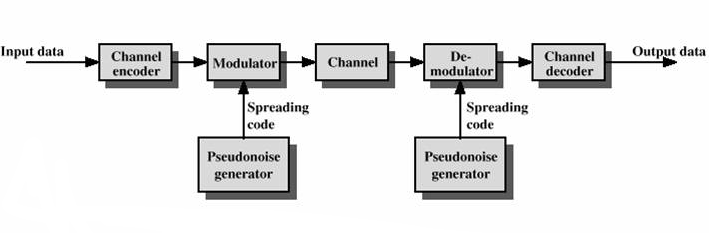
\includegraphics[width=2.5in]{fhss.png}
\text{Fig. 1 Frequency Hopping Spread Spectrum block diagram}
\end{center}
%\label{fig_sim}
%\end{figure}

This predefined, ordered mapping of frequency and duration is referred to as the frequency hopping pattern (FHP).
Using a FHP, transmission errors due to interference are lessened since the affected channel will only be transmitted on for a brief period.
If part of the band is being jammed, only the data sent along that part of the band is lost; while the rest of the channels remain unaffected.
Additionally, it is more difficult for an attacker to listen to communication on a frequency hopping system if they do not know the FHP.
This style of communication also lends well to multiple devices communicating at once.
Only when the pattern of two devices involve transmitting on the same frequency does a chance for collision occur.

The implementations of FHSS are nearly countless, and it is so incredibly common that is has reached a point of ubiquity.
Due to its obvious advantages, it is used in both commercial and military environments.
Some notable examples of frequency hopping in daily life are IEEE's 802.11 standard (Wi-Fi), and bluetooth (albeit with adaptive frequency hopping spread spectrum or AFH).

There is much study into the field of pattern recognition for FHSS.
By monitoring a given band, it is possible to derive the FHP.
Once the pattern is obtained, eavesdropping on the communication becomes consistent and easy.
The third-party need only tune its receiver to the appropriate channel during the known duration.
Alternatively, one can follow the FHP and jam each frequency [3] to completely disrupt communication.
This particular application has its use for military operations.

An interesting and common complication with detecting a FHP over a frequency band is the case of multiple sender with different FHP sending at once.

\section{Problem Statement}

The goal of this project is to be able to model a wireless system which uses FHSS, be able to generate a FHP, and then be able to detect the FHP with little to no prior knowledge from the perspective of an unknown third-party.
This will involve some mathematical modeling, as well as a programming simulation to test the results.
As such, there are several important steps necessary to complete this project.

First, we will need to find a way to model the wireless medium.
At minimum, the model must be able to simulate communication over several channels, with the ability for receivers to listen on different channels (not just the one being transmitted over).

After we have created our model, we will create a way to simulate communication over the virtual, wireless medium.
To start, we will not be simulating actual symbols or messages, as this will lead to more edge cases for the detector.
Rather, it will be a binary operation in which a given channel is either (1) being transmitted on or (0) not being transmitted on.

Next, we need to generate the FHP.
This is pretty straightforward.
We will feed the generator our parameters including: number of channels, minimum duration, and maximum duration.
For the purposes of this project, the generator will use each frequency exactly one time in the pattern.

Next, we will need to create and distribute a shared FHP between the sender, and receiver.
This FHP will have its own set of constraints and assumptions.
The two most notable will be the maximum transmission duration, and the number of channels.

Then, we will need to create a pattern detection scheme for use with an eavesdropping third-party.
This will be the mathematical side of the project.
Ideally, the model will be constructed in such a way that multiple schemes can be tested at once.
This would allow a good base of reference for future schemes, and give us relative results quickly.


\section{Solutions}

This project is split into the aforementioned parts.
We will discuss them in the order in which they were introduced: first the simulation, then the pattern generation, and then finally the pattern detection.
First, however, we will explore the assumptions and thoughts I have about the simulation.

\subsection{Assumptions}

First, the simulation will not be real time.
Efforts were made to make the simulation work in real-time, but this proved to be impossible.
Due to the way scheduling works on operating systems, there is no guarantee that the pattern will be executed in exactly the length of time desired.
In practice, the execution time varies by about +/- 5\% per pattern iteration.
This was too inconsistent for the simple pattern recognition schemes we are looking at, and accounting for this shifting pattern was deemed to be outside of the scope of this project.
Therefore, we will use discrete blocks to represent the real-world time units instead of milliseconds.
This gives us the ability to take our time with processing and not worry about the real-world limitations of the individual processor that the detector is being run on.
Specifically, we will be considering a single time block to be the time for a single frame to transmit.

Additionally, this simulation will work with discrete frequency values, represented as numbered channels.
This is to remove unfortunate difference in the discrete world of the computer and a real wireless system.
As an example, setting the discrete receiver to listen to the third channel on the 2.4Hz band could easily result in issues regarding \textit{double} values in C++.
This same issue is not as present in analog systems, where the receiver would pick up communication within some threshold from the center frequency.

Finally, the sender will transmit constantly and indefinitely.
To make detection more straightforward (at least for now) the sender should not stop sending.
In a real system, the sender will stop transmitting if it has nothing to say, but this complication makes detecting the correct pattern much more difficult.
Also, the whether or not the sender was communicating would then need to be psuedo-random and so the performance of the detector could be affected by chance.

\subsection{Implementation in C++}

To implement the model in code, I have chosen to use C++.
We will now explore each class to see how they will allow us to adequately simulate a real wireless system. 

\subsubsection{Medium}

This class models the functionality of the actual communication medium.
For this project, the medium which is being modeled is wireless system.
The medium is shared among all senders and receivers via the controller.
The medium has only a few variables and functions, primarily keeping track of which single channel is currently active.

\subsubsection{Controller}

Due to our discrete time blocks, we are able to execute the entire system on a single thread.
This massively reduced the complexity of the design, and gave rise to the controller and request system.
At the beginning of each time block, each device is polled for its desired operation, starting with the sender.
The devices can \textit{Send}, \textit{Listen}, or perform no operation (\textit{NOOP}).
It is the job of the controller to fulfill the requests of each device and increment the time block.

\subsubsection{PatternGenerator}

The \textit{PatternGenerator} class is responsible for generating the FHP.
This pattern is shared with the \textit{Sender}, and is meant to be derived by the \textit{PatternDetector}.
For a given number of channels, and the minimum and maximum time units, a psuedo-random, ordered \textit{vector} of \textit{pairs} is created.
The \textit{pair} consists of the channel to transmit on, and the duration to transmit for.
Since the pattern is a predetermined, finite sequence, it will be shared in its entirety rather than sharing (as an example) a seed or key for generating the pattern.

\subsubsection{Sender}

The \textit{Sender} class uses the generated pattern to continuously transmit over the medium.
An important note is that there are no actual communications sent.
Instead, the \textit{Sender} updates \textit{Controller} with the channel that should be considered active next.
After the corresponding duration has elapsed, the \textit{Sender} updates the \textit{Controller} that the channel is no longer active.
This continues for the entire FHP, and loops indefinitely.
As noted above, the communication is also entirely simulated.
There are no symbols or bits being sent, rather a binary state of the channel.

\subsubsection{PatternDetector}

The \textit{PatternDetector} class must derive the FHP by only interfacing with the Medium via the Controller.
The only operation available to it is polling the Medium to determine if the given channel is active.
Using just this, it should be able to implement the mathematical model, and ultimately arrive at the correct FHP.


\subsection{Pattern Detection Models}

Two models were considered for deriving the FHP.
Though they share similarities, the way they operate quite differently.

\subsubsection{Burst Detector}

The idea behind the burst detector is to use the knowledge that multiple, sequential time slots will be on the same channel.
This detector looks for these channel bursts and uses them to derive the pattern.

The burst detector begins by listening on a single channel until its starting frequency is heard (in our case, this is channel 0).
The detector then waits for the burst currently executing to end in order to gain the starting point.
Once the channel is no longer active, the counter begins to increment its internal count for each time slot that the channel is inactive.
When the channel is again active, the detector continues to increment until the channel goes inactive for a second time.
This gives us the entire pattern's length; a good starting place.
Additionally, the first frequency is pushed to the back of the detector's internal frequency vector.
This vector, with its pair the duration vector, keep track of the determined frequencies and duration.

Next, the detector must derive the duration associated with the first frequency.
This is done by again waiting until the channel is active, and then counting the number of time slots until the channel is inactive.

Once this duration is acquired, the detector begins to alternate finding frequencies and their duration.
The next frequency is determined by guessing what the next frequency will be after the last known value.
If the guess is incorrect, it waits until the pattern loops and tries again with a new guess.
This continues until the guess is correct and a new frequency can be pushed to the frequency vector.

The duration is determined much the same way as the initial; by counting how long until the channel becomes inactive.

Once the entire pattern length is accounted for, the pattern is considered detected and the detector begins requesting \textit{NOOP}s until the system stops running.

\subsubsection{Puzzle Piece Detector}

The puzzle piece detector works a bit differently from the burst detector.
Instead of keeping track of frequencies and durations separately, this detector creates a vector with a size the same as the pattern's length in time slots.
Every entry of this vector is initialized to an invalid channel number, and is filled as the detector operates.
The general idea, is that the detector keeps another vector of possible pieces in each time slot.
Pieces are tried sequentially and removed if found to not "fit" in the puzzle.
Once every entry in the puzzle has a valid frequency, the pattern is considered to be detected.

First, the pattern's length is determined in the same way as the burst detector.
Once the length is determined, the puzzle vector and two dimensional pieces vector are initialized.

For each time slot, the detector requests to listen on the next channel in the pieces vector at the corresponding index.
If the channel is heard, the puzzle is updated, and the detector will continue to listen until the channel is inactive; updating the whole time.
When the channel is not heard, that frequency is removed as a "piece" from the corresponding pieces vector element, and will not be tested again.

\section{Results and Analysis}

For each test, both detectors were run on the same pattern simultaneously.
This allowed for fair comparison without bias due to the psuedo-random pattern.

\subsection{Burst Detector}


\subsubsection{Results}
The results from five tests with ten channels can be seen in Figure 2.
The detector was successful in deriving the pattern each time it was run.
It took between 30 and 40 pattern iterations for the detector to derive the pattern.

The detector was tested with various pattern duration and channel numbers, and it was still able to derive the pattern.

\begin{center}
\begin{tabular}{|c|c|c|}
\hline
\text{Attempt} & \text{Time Slots for Detection} & \text{Pattern Iterations} \\
\hline
1 & 15,331 & 37.21 \\
\hline
2 & 16,979 & 41.21 \\
\hline
3 & 15,253 & 37.02 \\
\hline
4 & 13,231 & 32.11 \\
\hline
5 & 13,139 & 31.89 \\
\hline
\end{tabular}

\text{Fig. 2. Burst Detector Results}
\end{center}

\subsubsection{Analysis}

The burst detector was faster than originally expected.
Due to the large amount of downtime, one would think that the detector would take much longer to run.
However, the detector is uniquely able to rule out entire channels once they have been found in the pattern.
This means that the detector starts slow, but quickly speeds up as channels are eliminated.

Another point in the favor of this detector is its low spatial complexity.
The detector uses only two vectors to keep track of the order of frequency and duration respectively.
This means that this detector can easily be implemented on even the smallest of controllers.

\subsection{Puzzle Piece Detector}


\subsubsection{Results}
The results from five tests with ten channels can be seen in Figure 3.
the detector was successful in deriving the pattern each time it was run.
It took between 11 and 12 pattern iterations for the detector to derive the pattern.

\begin{center}
\begin{tabular}{|c|c|c|}
\hline
\text{Attempt} & \text{Time Slots for Detection} & \text{Pattern Iterations} \\
\hline
1 & 4,661 & 11.31 \\
\hline
2 & 4,661 & 11.31 \\
\hline
3 & 4,551 & 11.05 \\
\hline
4 & 4,618 & 11.21 \\
\hline
5 & 4,944 & 12.00 \\
\hline
\end{tabular}

\text{Fig. 3. Puzzle Piece Detector Results}
\end{center}

\subsubsection{Analysis}

First, this detector was significantly faster than the burst detector.
This was likely due to this detector's constant learning.
Where the other detector needed to wait for a new pattern iteration to try a different channel, this detector was able to gain new information all the time.

This speed does come at a cost, however.
The burst detector only needed two vectors (one for frequency, one for duration) and a count of the length of the current burst.
This detector, however, was significantly more spatially complex.
The puzzle vector is the same length as the total pattern duration in slots.
Then, the pieces vector is the same size as the puzzle vector, but with another dimension which is the same size as the number of channels.
In this case, the extra space was not an issue due to the small channel size, pattern duration, and large amount of storage on the host machine.
One can imagine, however, that a sufficiently large number of channels and large pattern length could create an unwieldy amount of space to be consumed.
This could especially be a problem if the detector is implemented on an embedded controller.

The detector could have been improved a good deal.
Since it only ever guessed the next channel sequentially based on previous guesses for that time slot, it would often guess at impossible choices.
A fix for this would have been to rule out certain channels.
For example, if the pattern had the following puzzle segment: 3, 3, 3, 3, 5, 5, 2, 2, 2, 2 then the detector could reasonably not guess that channel 5 is active anywhere else in the pattern.

\section{Conclusions}

Both detectors were successful.
One had low spatial complexity, at the expense of greater time complexity, and the other had low time complexity at the expense of greater spatial complexity.
Overall, the results were satisfying.
That said, both detectors could have been improved.

The burst detector did spend too much time idle.
Once the detector guessed incorrectly, it should have kept searching to find the next potential channel.
There is no guarantee that the next active channel it listened to would come next in the pattern, but this information could prove useful.

The puzzle piece detector could have calculated more likely next pieces, rather than going sequentially.
By looking backwards and forwards, the detector could have ruled out certain pieces, or given preference to more likely pieces.

Overall, I am pleased with the results.

\begin{thebibliography}{00}

\bibitem{b1} Y. Wang, Y. Lin, and X. Chi, `` Parameter Estimation Method of Frequency Hopping Signal Based On Sparse Time-frequency Method,'' 2018 IEEE 23rd International Conference on Digital Signal Processing (DSP), Nov. 2018.

\bibitem{b2} K.-G. Lee and S.-J. Oh, “Detection of Fast Frequency-Hopping Signals Using Dirty Template in the Frequency Domain,” IEEE Wireless Communications Letters, vol. 8, no. 1, pp. 281–284, Feb. 2019.

\bibitem{b3} X. Fan and Z. Tan, “Simulink Implementation of Frequency-hopping Communication System and Follower Jamming,” 2018 IEEE International Conference on Automation, Electronics and Electrical Engineering (AUTEEE), Nov. 2018. 

\bibitem{b4} X. Ning, S. Peng, and Z. Wang, “A Novel Anti-interference Scheme of Message-Driven Frequency Hopping Systems,” 2020 IEEE 3rd International Conference on Information Systems and Computer Aided Education (ICISCAE), 2020. 

\end{thebibliography}

\end{document}
